\documentclass[tikz,border=10pt]{standalone}
\usepackage{amsmath}
\usetikzlibrary{decorations.markings, positioning, arrows.meta, decorations.pathmorphing}

\begin{document}
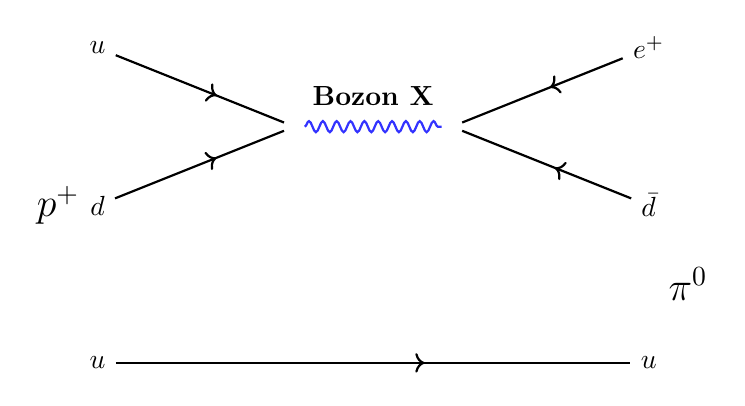
\begin{tikzpicture}[
    thick,
    fermion/.style={draw=black, postaction={decorate}, decoration={markings, mark=at position 0.6 with {\arrow{>}}}},
    antifermion/.style={draw=black, postaction={decorate}, decoration={markings, mark=at position 0.6 with {\arrow{<}}}},
    boson/.style={draw=blue!80, decorate, decoration={snake, amplitude=2pt, segment length=5pt}},
]

% Pozycje
\node (u1) at (0, 2) {$u$};
\node (d1) at (0, 0) {$d$};
\node (u2) at (0, -2) {$u$};
\node (v1) at (2.5, 1) {};
\node (v2) at (4.5, 1) {};
\node (e) at (7, 2) {$e^+$};
\node (dbar) at (7, 0) {$\bar{d}$};
\node (u2_out) at (7, -2) {$u$};

% Linie
\draw[fermion] (u1) -- (v1);
\draw[fermion] (d1) -- (v1);
\draw[boson] (v1) -- node[above=4pt] {\textbf{Bozon X}} (v2);
\draw[antifermion] (v2) -- (e);
\draw[antifermion] (v2) -- (dbar);
\draw[fermion] (u2) -- (u2_out);

% Klamry (zastępujemy prostymi tekstami jeśli brakuje bibliotek)
\node at (-0.5, 0) {\Large $p^+$};
\node at (7.5, -1) {\Large $\pi^0$};

\end{tikzpicture}
\end{document}
